 % use the "wcp" class option for workshop and conference
 % proceedings
 %\documentclass[gray]{jmlr} % test grayscale version
 %\documentclass[tablecaption=bottom]{jmlr}% journal article
 \documentclass[tablecaption=bottom,wcp]{jmlr} % W&CP article

 % The following packages will be automatically loaded:
 % amsmath, amssymb, natbib, graphicx, url, algorithm2e

 %\usepackage{rotating}% for sideways figures and tables
 %\usepackage{longtable}% for long tables

 % The booktabs package is used by this sample document
 % (it provides \toprule, \midrule and \bottomrule).
 % Remove the next line if you don't require it.
\usepackage{booktabs}
 % The siunitx package is used by this sample document
 % to align numbers in a column by their decimal point.
 % Remove the next line if you don't require it.
\usepackage[load-configurations=version-1]{siunitx} % newer version
\usepackage{bm}
 %\usepackage{siunitx}
 
 \definecolor{forestgreen}{rgb}{0.13, 0.55, 0.13}

\usepackage{pifont}
\newcommand{\cmark}{\color{forestgreen}{\ding{51}}}
\newcommand{\xmark}{\color{red}{\ding{55}}}


 % Define an unnumbered theorem just for this sample document for
 % illustrative purposes:
\theorembodyfont{\upshape}
\theoremheaderfont{\scshape}
\theorempostheader{:}
\theoremsep{\newline}
\newtheorem*{note}{Note}

% Our packages
\usepackage{listings}
\lstdefinelanguage{julia}
{
  keywordsprefix=\@,
  morekeywords={
    exit,whos,edit,load,is,isa,isequal,typeof,tuple,ntuple,uid,hash,finalizer,convert,promote,
    subtype,typemin,typemax,realmin,realmax,sizeof,eps,promote_type,method_exists,applicable,
    invoke,dlopen,dlsym,system,error,throw,assert,new,Inf,Nan,pi,im,begin,while,for,in,return,
    break,continue,macro,quote,let,if,elseif,else,try,catch,end,bitstype,ccall,do,using,module,
    import,export,importall,baremodule,immutable,local,global,const,Bool,Int,Int8,Int16,Int32,
    Int64,Uint,Uint8,Uint16,Uint32,Uint64,Float32,Float64,Complex64,Complex128,Any,Nothing,None,
    function,type,typealias,abstract
  },
  sensitive=true,
  morecomment=[l]{\#},
  morestring=[b]',
  morestring=[b]" 
}

\definecolor{mygray}{RGB}{128,128,128}
\definecolor{myblue}{RGB}{0, 0, 255}
\definecolor{myolivegreen}{RGB}{186, 184, 108}
\definecolor{mymaroon}{RGB}{128, 0, 0}


\lstset{
    language=julia,
    basicstyle=\small\ttfamily, 
    columns=fullflexible, % make sure to use fixed-width font, CM typewriter is NOT fixed width
    numbers=left, 
    numberstyle=\small\ttfamily\color{mygray},
    stepnumber=1,              
    numbersep=10pt, 
    numberfirstline=true, 
    numberblanklines=true, 
    tabsize=4,
    lineskip=-1.5pt,
    extendedchars=true,
    breaklines=true,        
    keywordstyle=\color{myblue}\bfseries,
    identifierstyle=, % using emph or index keywords
    commentstyle=\sffamily\color{myolivegreen},
    stringstyle=\color{mymaroon},
    showstringspaces=false,
    showtabs=false,
    upquote=false
}

\usepackage{adjustbox}
\usepackage{multirow}

\def\ahmc{\texttt{AHMC}}
\def\ahmcfull{\texttt{AdvancedHMC.jl}}
\def\stan{\texttt{Stan}}
\def\turing{\texttt{Turing}}
\def\turingjl{\texttt{Turing.jl}}

%%%

\jmlrproceedings{AABI 2019}{2nd Symposium on Advances in Approximate Bayesian Inference, 2019}

 % The optional argument of \title is used in the header
 
%  OLD / CURRENT TITLE.
\title[AdvancedHMC.jl:\\\large A modular implementation of Stan's No-U-Turn sampler]{AdvancedHMC.jl:\\\large A modular implementation of Stan's No-U-Turn sampler in Julia}

% \title[\ahmcfull: Modular State-of-the-Art HMC]{\ahmcfull: Modular State-of-the-Art HMC}

 % Anything in the title that should appear in the main title but 
 % not in the article's header or the volume's table of
 % contents should be placed inside \titletag{}

 %\title{Title of the Article\titletag{\thanks{Some footnote}}}


 % Use \Name{Author Name} to specify the name.
 % If the surname contains spaces, enclose the surname
 % in braces, e.g. \Name{John {Smith Jones}} similarly
 % if the name has a "von" part, e.g \Name{Jane {de Winter}}.
 % If the first letter in the forenames is a diacritic
 % enclose the diacritic in braces, e.g. \Name{{\'E}louise Smith}

 % \thanks must come after \Name{...} not inside the argument for
 % example \Name{John Smith}\nametag{\thanks{A note}} NOT \Name{John
 % Smith\thanks{A note}}

 % Anything in the name that should appear in the title but not in the 
 % article's header or footer or in the volume's
 % table of contents should be placed inside \nametag{}

% Anonymous authors (leave as is; do not reveal author names for your submission)
\author{\Name{Anonymous Authors}\\
  \addr Anonymous Institution}
% THE SUBMISSION MUST REMAIN ANONYMOUS

% Two authors with the same address
% \author{\Name{Author Name1\nametag{\thanks{A note}}} \Email{abc@sample.com}\and
%  \Name{Author Name2} \Email{xyz@sample.com}\\
%  \addr Address}

 % Three or more authors with the same address:
 % \author{\Name{Author Name1} \Email{an1@sample.com}\\
 %  \Name{Author Name2} \Email{an2@sample.com}\\
 %  \Name{Author Name3} \Email{an3@sample.com}\\
 %  \Name{Author Name4} \Email{an4@sample.com}\\
 %  \Name{Author Name5} \Email{an5@sample.com}\\
 %  \Name{Author Name6} \Email{an6@sample.com}\\
 %  \Name{Author Name7} \Email{an7@sample.com}\\
 %  \Name{Author Name8} \Email{an8@sample.com}\\
 %  \Name{Author Name9} \Email{an9@sample.com}\\
 %  \Name{Author Name10} \Email{an10@sample.com}\\
 %  \Name{Author Name11} \Email{an11@sample.com}\\
 %  \Name{Author Name12} \Email{an12@sample.com}\\
 %  \Name{Author Name13} \Email{an13@sample.com}\\
 %  \Name{Author Name14} \Email{an14@sample.com}\\
 %  \addr Address}


 % Authors with different addresses:
 % \author{\Name{Author Name1} \Email{abc@sample.com}\\
 % \addr Address 1
 % \AND
 % \Name{Author Name2} \Email{xyz@sample.com}\\
 % \addr Address 2
 %}



\begin{document}

\maketitle

% Will: have given the abstract another pass to try and sell it a bit more. Please feel free to modify / revert etc.

% \begin{abstract}
% The No-U-Turn Sampler (NUTS) in \stan \citep{hoffman2014no,carpenter2017stan} has demonstrated remarkable sampling robustness and efficiency in a wide range of Bayesian inference problems due to the use of dynamic Hamiltonian trajectory and a fine-tuned windowed adaptation of step-size and mass matrix. Motivated by these successes, we present \ahmcfull (\ahmc), a pure Julia implementation of \stans built-in NUTS algorithm and related adaptation methods. We hope \ahmc can help expose \stans NUTS to a wider range of users, e.g. those who want to write their models by hand or use a different probabilistic programming language, such as \turing or \texttt{Soss}. In our package, NUTS is defined as a composition of individual components with abstractions partially inspired by \citet{betancourt2017conceptual}. As being pure Julia, \ahmc also runs on GPUs by utilising \texttt{CuArrays.jl}.
% \end{abstract}
% \texttt{AdvancedHMC.jl}
\begin{abstract}
 Stan's Hamilton Monte Carlo (HMC) has demonstrated remarkable sampling robustness and efficiency in a wide range of Bayesian inference problems through carefully crafted adaption schemes to the celebrated No-U-Turn sampler (NUTS) algorithm.  It is challenging to implement these adaption schemes robustly in practice, hindering wider adoption amongst practitioners who are not directly working with the Stan modelling language. AdvancedHMC.jl (AHMC) contributes a modular, well-tested, standalone implementation of NUTS that recovers and extends Stan's NUTS algorithm. AHMC is written in Julia, a modern high-level language for scientific computing, benefiting from optional hardware acceleration and interoperability with a wealth of existing software written in both Julia and other languages, such as Python. Efficacy is demonstrated empirically by comparison with Stan through a third-party Markov chain Monte Carlo benchmarking suite.
\end{abstract}

% Keywords may be removed
%\begin{keywords}
%List of keywords
%\end{keywords}

\section{Introduction}
\label{sec:intro}

Hamiltonian Monte Carlo (HMC) is an efficient Markov chain Monte Carlo (MCMC) algorithm which avoids random walks by simulating Hamiltonian dynamics to make proposals \citep{duane1987hybrid,neal2011mcmc}. Due to the statistical efficiency of HMC, it has been widely applied to fields including physics \citep{duane1987hybrid}, differential equations \citep{kramer2014hamiltonian}, social science \citep{jackman2009bayesian} and Bayesian inference \citep[e.g. Bayesian neural networks;][]{neal2012bayesian}. The No-U-Turn Sampler \citep[NUTS;][]{hoffman2014no} is an extension of the HMC sampler which automatically tunes two key parameters, the leapfrog step size and integration time (aka trajectory length), which used to require manual adjustments through extensive preliminary runs. Together with a robust implementation in the \stan\, probabilistic programming language (PPL), NUTS has become the default choice for HMC sampling for many probabilistic modelling practitioners \citep{carpenter2017stan}.

% Although the black-box nature of \stans\, NUTS makes Bayesian inference easy for those domain experts happy to use \stan, it does not provide a satisfactory solution for researchers and practitioners not working in the \stan\, ecosystem. AdvancedHMC.jl provides a robust implementation of state-of-the-art algorithms that are easily utilised in a range of programming languages, are not tied to a particular PPL, and can be used to facilitate research into improved HMC algorithms.

Although the black-box nature of \stan's NUTS makes Bayesian inference easy for domain experts relying on %happy to use 
\stan, it is desirable to have a high quality NUTS implementation in a high-level language, 
%for e.g.: research on 
e.g.~for research on HMC algorithms, reproducible comparisons and real-world approximate inference applications. To this end, we introduce \ahmcfull ~(\ahmc), a robust, modular and efficient implementation of \stan's NUTS and several other commonly used HMC variants in Julia.\footnote{Code is available at \url{https://anonymous.4open.science/r/27c8d4a6-8ee3-452a-8a63-db8fb3408182/}.}

\section{A modular HMC library}

%% I don't understand this sentence. What?
\ahmc~supports various HMC algorithms in the set below resulted from a Cartesian product of a set of HMC trajectories and a set of adaptors:
$$
(\texttt{StaticTrajectory}\; \cup\; \texttt{DynamicTrajectory}) \times \texttt{Adaptor}.
$$
%% A set or the set?
Here $\texttt{StaticTrajectory}$ refers to a set of HMC with fixed-length trajectory length, which contains HMC with fixed step size and step numbers and HMC with fixed total trajectory length. $\texttt{DynamicTrajectory}$ is a set of HMC with adaptive trajectory length 
which is defined as a Cartesian product of four sets of different HMC components:
$$
\texttt{Metric} \times \texttt{Integrator} \times \texttt{TrajectorySampler} \times \texttt{TerminationCriterion},
$$
where 
\begin{align*} 
    \texttt{Metric} &=  \{ \texttt{UnitEuclidean}, \texttt{DiagEuclidean}, \texttt{DenseEuclidean} \} \\ 
    \texttt{Integrator} &=  \{ \texttt{Leapfrog}, \texttt{JitteredLeapfrog}, \texttt{TemperedLeapfrog} \} \\
    \texttt{TrajectorySampler} &=  \{ \texttt{Slice}, \texttt{Multinomial} \} \\
    \texttt{TerminationCriterion} &= \{ \texttt{ClassicNoUTurn}, \texttt{GeneralisedNoUTurn} \}
\end{align*}
Finally, $\texttt{Adaptor}$ consists of any $\texttt{BaseAdaptor}$ or any composition of two or more $\texttt{BaseAdaptor}$, where $\texttt{BaseAdaptor} \in \{\texttt{Preconditioner}, \texttt{NesterovDualAveraging}\}$.
% $\texttt{Preconditioner}$ behaves differently based on the choice of metric spaces. 
A special composition called $\texttt{StanHMCAdaptor}$ is provided to compose \stan's windowed adaptor, which has been shown to be robust in practice 
%in \stan\;
\citep{carpenter2017stan}.

\subsection{Example code of building \stan's NUTS using \ahmcfull}
%% To illustrate instead of show?
%% Maybe: 
The code snippet below illustrates the use of \ahmc~for a given target log density function and its gradient, \texttt{logdensity\_f} and \texttt{grad\_f} respectively.
% To show the interface of \ahmc, we provide a code snippet of building \stan's NUTS. 
\lstinputlisting{example.jl}
%% Maybe: Note that \texttt{logdensity\_f} can be derived from an independent PPL, manually defined or given by a normalising flow.
Here \texttt{logdensity\_f} and \texttt{grad\_f} are functions of the target distributions's log density and its gradient, which are functions independent of \ahmc~and can be, e.g. derived from different PPLs or defined by normalising flows \citep{Rezende2015-yo,dinh2016density,papamakarios2017masked}. We will show an example of such models in the next section.

\subsection{GPU support for \ahmcfull~via \texttt{CuArrays.jl}}
%% Hm, I would rephrase this and move this sentence below the next one.
In order to run HMC on CUDA, 
one only needs to change Line 3 of the demo code 
from \texttt{q0 = randn(D)} to \texttt{q0 = CuArray(randn(D))}, 
assuming \texttt{logdensity\_f} and \texttt{grad\_f} in Line 6 are GPU friendly, which is how \texttt{CuArrays.jl} could be used with \texttt{AdvancedHMC.jl} to run HMC on GPUs.
An example using GPU accelerated \ahmc\;to draw samples from a normalising flow, named \texttt{flow\_model}, trained on MNIST \citep{lecun1998mnist} is given below. The function \texttt{logpdf(m, x)} is used to compute the log density for model \texttt{m} on data batch \texttt{x}.
% if it is written in pure Julia, it probably supports GPUs acceleration automatically.

\lstinputlisting{gpu.jl}

Here \texttt{Tracker} is an automatic differentiation (AD) library which implements reverse-mode AD.
\textit{How does it work?}
All arrays in \ahmc~are abstractly typed, meaning that the concrete type is deduced at compile time from \texttt{q0}. That is to say, if \texttt{q0} is defined on the GPU, i.e.~it is a \texttt{CuArray}, all internal arrays in HMC will be too.

\section{Related work}
A summary of the related work on HMC/NUTS implementations is given in Table~\ref{tb:related-work} in the appendix.
%Here \textit{modern NUTS} refers to the use of multinominal sampling for trajectories and the use of generalised no-U-turn criterion. Multinominal sampling has been proven to give significant improvement on statistical efficiency for NUTS in \stan compared with slice sampling \citep{betancourt2017conceptual}.
We want to emphasis that there exists a Python API of \ahmc~implemented by an independent team available at \url{https://github.com/salilab/hmc}.
%

%\begin{table}[t]
%\caption{Comparison of different HMC/NUTS implementations.}
%\label{tb:related-work}
%\centering
%\scalebox{0.9}{
%\begin{tabular}{lllll}
%\toprule
%        & Compositional & Modern NUTS & GPU support & External %API \\
%\midrule
%\stan    &      NO     &     YES      &      YES   &   NO      %\\
%\texttt{Edward2} &      NO     &     YES      &     YES     &  %     YES       \\
%\texttt{PyMC3}   &       NO      &     YES      &      YES    & %    NO     \\
%\texttt{Pyro}   &       NO      &     NO      &     YES     &  %   YES     \\
%\ahmc    &      YES     &    YES      &    YES     &     YES   % \\
%\bottomrule
%\end{tabular}
%}
%\vspace{-0.2in}
%\end{table}



%%%


\section{Evaluations}
To compare the NUTS implementation between \ahmc~ and \texttt{Stan}, we consider five models from \texttt{MCMCBenchmarks.jl}, a package for benchmarking MCMC libraries in Julia.\footnote{Available at \url{https://github.com/StatisticalRethinkingJulia/MCMCBenchmarks.jl}.} The five models are 1) a \textit{Gaussian model} (Gaussian), a simple two parameter Gaussian distribution, 2) the \textit{signal detection model} (SDT), a model used in psychophysics and signal processing \citep{green1966signal}, 3) a \textit{linear regression} model (LR), 4) a \textit{hierarchical Poisson regression} (HPR) model and 5) the \textit{linear ballistic accumulator model} (LBA), a cognitive model of perception and simple decision making \citep{brown2008simplest}. Please refer to Appendix~\ref{app:models} for full descriptions of these models.

\subsection{Statistical property of simulated trajectories}
To compare the statistical property between \texttt{Stan} and \texttt{AHMC},
we run multiple chains of NUTS with target acceptance rate $0.8$ 
for $2,000$ steps with $1,000$ for adaptation,
where the warm-up samples are dropped.
Each model is benchmarked with multiple data sizes $N$.
We compare the simulated trajectories by the distributions of step size and tree depth and the average effective sample size (ESS) for all variables. The results for the SDT model is shown in Figure~\ref{fig:sdt}.
\begin{figure}[t]
    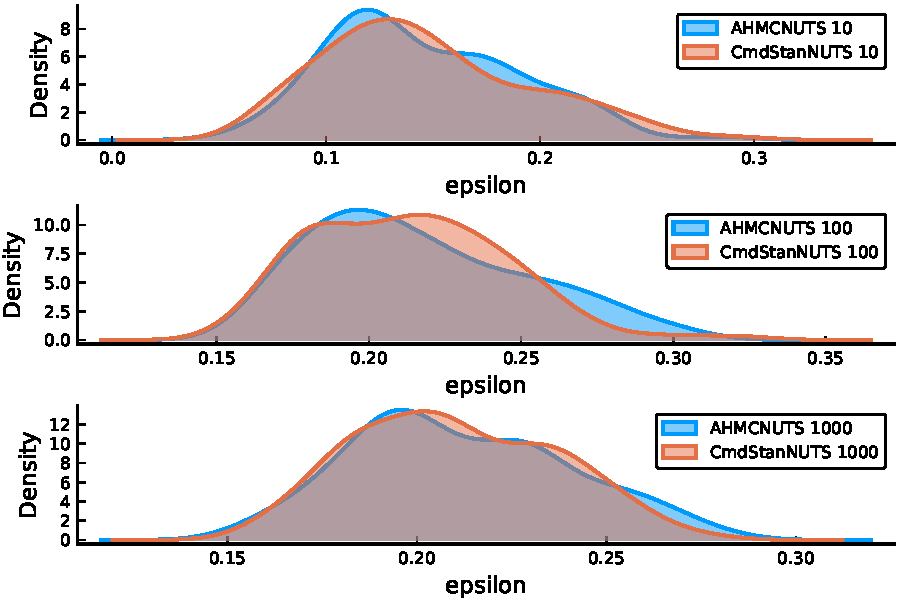
\includegraphics[width=0.3\textwidth]{images/Linear_Regression/density_epsilon.pdf}
    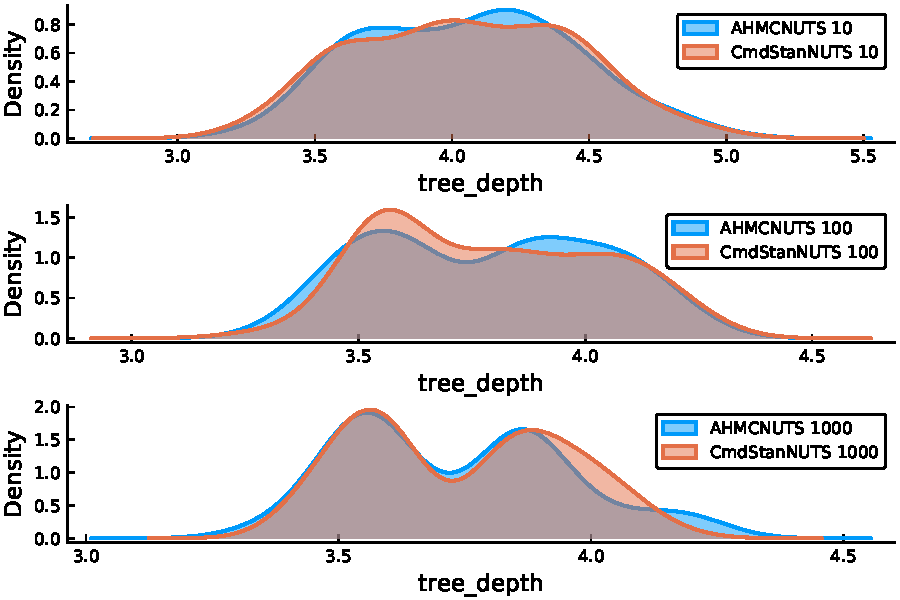
\includegraphics[width=0.3\textwidth]{images/Linear_Regression/density_tree_depth.pdf}
    \;\hfill
    \raisebox{\height}{\scalebox{0.67}{
        \begin{tabular}{lrrrrr}
            \toprule
            \multirow{2}{*}{} & \multirow{2}{*}{$N$} & \multicolumn{4}{c}{ESS} \\
            & & \multicolumn{1}{c}{$b_0$} & \multicolumn{1}{c}{$\sigma$} & \multicolumn{1}{c}{$b_1$} & \multicolumn{1}{c}{$b_2$} \\
            \midrule
            \texttt{Stan} & 10 & 413.939 & 266.476 & 381.219 & 423.441 \\
            \texttt{AHMC} & 10 & 354.946 & 263.894 & 411.769 & 399.420 \\
            \texttt{Stan} & 100 & 621.796 & 729.812 & 465.990 & 608.608 \\
            \texttt{AHMC} & 100 & 473.005 & 734.189 & 606.996 & 621.543 \\
            \texttt{Stan} & 1000 & 668.524 & 789.987 & 464.459 & 648.201 \\
            \texttt{AHMC} & 1000 & 485.988 & 786.577 & 676.097 & 689.344 \\
            \bottomrule
        \end{tabular}
    }}
    \vspace{-0.25in}
    \caption{LR (50 runs). For the density plots, blue is for \ahmc~and orange is for \stan~and each row is for a different size $N$, corresponding to the table on the right.}
    \vspace{-0.2in}
\end{figure}
It can been seen that the distributions of step size and tree depth are similar and the average ESS for all variables are close, indicating \ahmc's NUTS is statistically similar to the implementation in \stan. 
%% This is a strange sentence. Maybe rephrase?
Conclusions from the results of the other four models remain similar; see Appendix~\ref{app:stat-prop} for figures and tables.

\subsection{Computational efficiency via running time}
All the benchmark models used in this paper are implemented in \turing~\citep{pmlr-v84-ge18b}, a universal PPL in Julia that
uses \ahmc~as its HMC backend; see Appendix~\ref{app:turing-lr} for an example \turing~code.
The average time used to run the five benchmark models for multiple times using \texttt{Stan} and using \texttt{AHMC} via \turing~are reported in Table~\ref{tb:time}.
\begin{table}[t]
\centering
\scalebox{0.9}{
\begin{tabular}{lrrrrrrrrrr}
    \toprule
0    %\multirow{2}{*}{} & \multicolumn{10}{c}{Data Size \& Mean Time (s)} \\
    & \multicolumn{2}{c}{Gaussian $^2$} & \multicolumn{2}{c}{SDT $^3$} & \multicolumn{2}{c}{LR $^2$} & \multicolumn{2}{c}{HPR $^1$} & \multicolumn{2}{c}{LBA $^2$} \\
    & \multicolumn{1}{c}{$N$} & \multicolumn{1}{c}{seconds} & \multicolumn{1}{c}{$N$} & \multicolumn{1}{c}{seconds} & \multicolumn{1}{c}{$N$} & \multicolumn{1}{c}{seconds}& \multicolumn{1}{c}{$N$} & \multicolumn{1}{c}{seconds}& \multicolumn{1}{c}{$N$} & \multicolumn{1}{c}{seconds} \\
    \midrule
    %\texttt{Stan} & 10 & 0.803881 & 10 & 0.775959 & 10 & 0.866924 & 10 & 2.487 & 10 & 1.91799 \\
    \texttt{Stan} & 10 & 0.8039 & 10 & 0.7759 & 10 & 0.8669 & 10 & 2.4870 & 10 & 1.9179 \\
    %Turing & 10 & 0.336073 & 10 & 0.328538 & 10 & 1.13563 & 10 & 19.4587 & 10 & 2.69062 \\
    \texttt{AHMC} & 10 & 0.3361 & 10 & 0.3285 & 10 & 1.1356 & 10 & 19.4587 & 10 & 2.6906 \\
    %\texttt{Stan} & 100 & 0.756092 & 100 & 0.726106 & 100 & 0.982419 & 20 & 3.50248 & 50 & 7.84705 \\
    \texttt{Stan} & 100 & 0.7561 & 100 & 0.7261 & 100 & 0.9824 & 20 & 3.5025 & 50 & 7.8471 \\
    %Turing & 100 & 0.33034 & 100 & 0.320111 & 100 & 1.32024 & 20 & 28.2982 & 50 & 11.027 \\
    \texttt{AHMC} & 100 & 0.3303 & 100 & 0.3201 & 100 & 1.3202 & 20 & 28.2982 & 50 & 11.0270 \\
    %\texttt{Stan} & 1000 & 0.761393 & 1000 & 0.708934 & 1000 & 2.26 & 50 & 5.89541 & 200 & 31.3762 \\
    \texttt{Stan} & 1000 & 0.7614 & 1000 & 0.7089 & 1000 & 2.2600 & 50 & 5.8954 & 200 & 31.3762 \\
    %Turing & 1000 & 0.508123 & 1000 & 0.317854 & 1000 & 3.83261 & 50 & 40.0322 & 200 & 33.6125 \\
    \texttt{AHMC} & 1000 & 0.5081 & 1000 & 0.3179 & 1000 & 3.8326 & 50 & 40.0322 & 200 & 33.6125 \\
    \bottomrule
\end{tabular}
}
\vspace{-0.05in}
\caption{Computational efficiency for five models using $^1$ 25 runs, $^2$ 50 runs or $^3$ 100 runs. For \ahmc, forward-mode AD is used for computing gradient. \ahmc~can be used together with different AD backends/packages, e.g.~\texttt{ForwardDiff.jl}'s forward-mode AD, \texttt{Tracker.jl}'s reverse-mode AD and \texttt{Zygote.jl}'s source-to-source AD.}
\label{tb:time}
\vspace{-0.30in}
\end{table}
We see that \ahmc~has comparable performance for all models except for HPR, which could be the result of the difference in the implementation of the probability mass function for the Poisson distribution. Also note that \ahmc~scales better for LBA models while \stan~scales better for the rest of the models. This is likely due to the fact that the LBA model relies on a manually implemented distribution which is highly optimized by Julia's compiler.
%% Hm, what is it.. optimised code or difference in AD? I would only mention one. The difference in the AD is applicable for all models, right?

\section{Conclusion}
% We presented a new software package named \ahmcfull~for robust, modular and efficient implementation of advanced HMC algorithms. %% Hm, hope doesn't sound very convincing.. .. hope hope... something else would be better.. 
% We hope \ahmc~can serve as a platform for research on HMC algorithms by providing a high-quality robust baseline. We also hope \ahmc~can make it easier to develop new probabilistic programming languages by decoupling inference algorithms and modelling language.%, such that programming language researchers can focus more on compiler-related innovations.
We have introduced \ahmcfull, a new Julia package that provides robust, modular and efficient implementations of advanced HMC algorithms. 
We highlight the modularity of the package and compare the implemented NUTS with \stan, both statistically and computationally.
Overall, we hope that AHMC can serve as a robust baseline for future research on HMC algorithms and can enable the development of new PPLs which take advantage of the decoupling of inference algorithms from the actual modelling language.
% \subsection{Easy Integration of Other Julia Packages}
% \texttt{Bijectors.jl} is used inside \texttt{Turing.jl} to do automatic transformations of constrained variables to run HMC. E.g. a random variable from $\mathcal{T}runcated(\mathcal{C}auchy(0, 5), 0, \infty)$ is constrained to be positive and will be transformed to the real space by the $\log$ function automatically. 


% \texttt{Soss.jl} is another PPL in Julia that
% uses \texttt{AdvancedHMC.jl} as its backend.
% It is easy for PPLs in Julia with different domain specific languages (DSLs)
% to use the HMC implementation in \texttt{AdvancedHMC.jl}.

% \texttt{DifferentialEquations.jl} is the state-of-the-art numerical differential equations solver package, implemented in pure Julia. As such, its solvers can be employed in Turing models, thus enabling \texttt{AHMC} to perform Bayesian inference in the parameters of differential equation models.

% \texttt{Flux.jl} is a deep learning packages in Julia.
% Neural models defined by \texttt{Flux.jl} can be directly used in Turing models.
% E.g. one can implement a Bayesian neural network in Turing by 
% defining priors on the weights of a Flux-based neural network, and 
% NUTS can be used to draw samples of the weights.

%%%

% \acks{We would like to thank the developers of \texttt{MCMCBenchmarks.jl}, Rob Goedman and Christopher Fisher.
%     With this package we ran all benchmarks and generated all plots presented in this paper.}


\bibliography{jmlr-sample}

\newpage

\appendix

\section{Related Work}
\begin{table}[htbp]
\label{tb:related-work}
    \floatconts
    {}
    {\caption{Comparison of different HMC/NUTS implementations. \texttt{TFP.MCMC} refers to \texttt{TensorFlow.Probability}'s MCMC library. \texttt{DynamicHMC} is another high-quality HMC implementation in Julia. Windowed adaption is a method for joint adaption of leapfrog integration step-size and mass matrix. Windowed adaption was proposed by the Stan team \citep{carpenter2017stan}, and has demonstrated remarkable robustness in a wide range of Bayesian inference problems. Partial support for GPU means the log density function can be accelerated by GPU, but the HMC sampler itself runs on CPU. Slice and Multinomial are two methods for sampling from dynamic Hamiltonian trajectories, e.g. those generated by the No-U-Turn algorithm (see e.g. \citet{betancourt2017conceptual} for details). Tempered leapfrog integrator improves convergence when the target distribution has multiple modes by performing tempering within Hamiltonian trajectories \citep{neal2011mcmc}.}}
    {
    \begin{tabular}{l|cccccc}
    & \texttt{Stan} & \texttt{AHMC} (ours) & \texttt{Pyro} & \texttt{TFP.MCMC} & \texttt{PyMC3} & \texttt{DynamicHMC} \\
    \hline
    % \multirow{3}{*}{Adaption}& 
    \textbf{Adaption} \\
    Step-size & \cmark  & \cmark & \cmark & \cmark & \cmark &\cmark \\
    Mass matrix & \cmark & \cmark & \cmark & \cmark & \cmark &\cmark \\
    Windowed adaption & \cmark & \cmark & \xmark & \xmark & \xmark & \cmark\\
    \hline
    % \multirow{3}{*}{Hamiltonian trajectory} & 
    \textbf{Hamiltonian trajectory} \\
    Classic No-U-Turn & \cmark & \cmark & \xmark & \cmark & \xmark &\xmark \\
    Generalised No-U-Turn & \cmark & \cmark & \cmark & \cmark & \cmark &\cmark \\
    Fixed trajectory length& \cmark & \cmark & \cmark & \cmark & \cmark & \xmark\\
    \hline
    % \multirow{2}{*}{Trajectory sampler} & 
    \textbf{Trajectory sampler} \\
    Slice & \cmark & \cmark & \cmark & \cmark & \xmark &\xmark \\
    Multinomial & \cmark & \cmark & \cmark & \cmark & \cmark &\cmark \\
    \hline
    % \multirow{3}{*}{Integrator}& 
    \textbf{Integrator} \\
    Leapfrog & \cmark &\cmark  & \cmark & \cmark & \cmark & \cmark\\
    Jittered Leapfrog & \cmark & \cmark & \xmark & \xmark & \xmark &\xmark \\
    Tempered Leapfrog & \xmark &\cmark  & \xmark & \xmark & \xmark & \xmark\\
    \hline
    GPU support & partial & \cmark & \cmark & \cmark & partial & partial \\
    % \hline
    \end{tabular}
    }
\end{table}

\section{Full descriptions of models used for evaluations}
\label{app:models}
Below are the full descriptions of five models used for evaluations.

\textbf{Gaussian Model (Gaussian)}
is a simple two parameter Gaussian distribution.
\begin{align}
    \mu &\sim \mathcal{N}(0, 1) \nonumber \\
    \sigma &\sim \mathcal{T}runcated(\mathcal{C}auchy(0, 5), 0, \infty) \nonumber \\
    y_n &\sim \mathcal{N}(\mu, \sigma) \; (n = 1, \dots, N) \nonumber
\end{align}
% $$
% \mu \sim \mathcal{N}(0, 1), \quad 
% \sigma \sim \mathcal{T}runcated(\mathcal{C}auchy(0, 5), 0, \infty), \quad
% y_n \sim \mathcal{N}(\mu, \sigma) \; (n = 1, \dots, N)
% $$

\textbf{Signal Detection Model (SDT)}
is a model used in psychophysics and signal processing, 
which decomposes performance in terms of discriminability and bias \citep{green1966signal}.
\begin{align}
d &\sim \mathcal{N}(0, \frac{1}{\sqrt{2}}) \nonumber \\
c &\sim \mathcal{N}(0, \frac{1}{\sqrt{2}}) \nonumber \\
x &\sim \text{SDT}(d, c) \nonumber
\end{align}
% $$
% d \sim \mathcal{N}(0, \frac{1}{\sqrt{2}}), \quad 
% c \sim \mathcal{N}(0, \frac{1}{\sqrt{2}}), \quad 
% x \sim \text{SDT}(d, c).
% $$

\textbf{Linear Regression Model (LR)}
is a linear regression with truncated Cauchy prior on the weights.
\begin{align}
    B_d &\sim \mathcal{N}(0, 10) \nonumber \\
    \sigma &\sim \mathcal{T}runcated(\mathcal{C}auchy(0, 5), 0, \infty) \nonumber \\
    y_n &\sim \mathcal{N}(\mu_n, \sigma) \nonumber
\end{align}
% $$
% B_d \sim \mathcal{N}(0, 10), \;
% \sigma \sim \mathcal{T}runcated(\mathcal{C}auchy(0, 5), 0, \infty), \;
% y_n \sim \mathcal{N}(\mu_n, \sigma),
% $$
where $\mu = B_0 + \bm{B}^T \bm{X}, d = 1, \dots, D$ and $n = 1, \dots, N$.

\textbf{Hierarchical Poisson Regression (HPR)}
\begin{align}
    a_0 &\sim \mathcal{N}(0, 10) \nonumber \\
    a_1 &\sim \mathcal{N}(0, 1) \nonumber \\
    b_\sigma &\sim \mathcal{T}runcated(\mathcal{C}auchy(0, 1), 0, \infty) \nonumber \\
    b_d &\sim \mathcal{N}(0, b_\sigma) \nonumber \\
    y_n &\sim \mathcal{P}oisson(\log\lambda_n) \nonumber
\end{align}
% $$
% a_0 \sim \mathcal{N}(0, 10), \;
% a_1 \sim \mathcal{N}(0, 1), \;
% b_\sigma \sim \mathcal{T}runcated(\mathcal{C}auchy(0, 1), 0, \infty), \;
% b_d \sim \mathcal{N}(0, b_\sigma), \;
% y_n \sim \mathcal{P}oi(\log\lambda_n),
% $$
where $\log\lambda_n = a_0 + b_{z_n} + a_1 x_n, d = 1, \dots, N_b$ and $n = 1, \dots, N$.

\textbf{Linear Ballistic Accumulator (LBA)}
is a cognitive model of perception and simple decision making \citep{brown2008simplest}.
\begin{align}
    \tau &\sim \mathcal{T}runcated(\mathcal{N}(0.4, 0.1), 0, mn) \nonumber \\
    A &\sim \mathcal{T}runcated(\mathcal{N}(0.8, 0.4), 0, \infty) \nonumber \\
    k &\sim \mathcal{T}runcated(\mathcal{N}(0.2, 0.3), 0, \infty) \nonumber \\
    \nu_d &\sim \mathcal{T}runcated(\mathcal{N}(0, 3), 0, \infty) \nonumber \\
    x_n &\sim \text{LBA}(\bm{\nu}, \tau, A, k) \nonumber
\end{align}
% $$
% \tau \sim \mathcal{T}runcated(\mathcal{N}(0.4, 0.1), 0, mn), \quad
% A \sim \mathcal{T}runcated(\mathcal{N}(0.8, 0.4), 0, \infty),
% $$
% $$
% k \sim \mathcal{T}runcated(\mathcal{N}(0.2, 0.3), 0, \infty), \quad
% \nu_d \sim \mathcal{T}runcated(\mathcal{N}(0, 3), 0, \infty), \quad
% x_n \sim \text{LBA}(\bm{\nu}, \tau, A, k)
% $$
where $mn=\min_i x_{i,2}, d = 1, \dots, N_c$ and $n = 1, \dots, N$.

\section{Statistical property of simulated trajectories}
\label{app:stat-prop}
\begin{figure}[h!]
    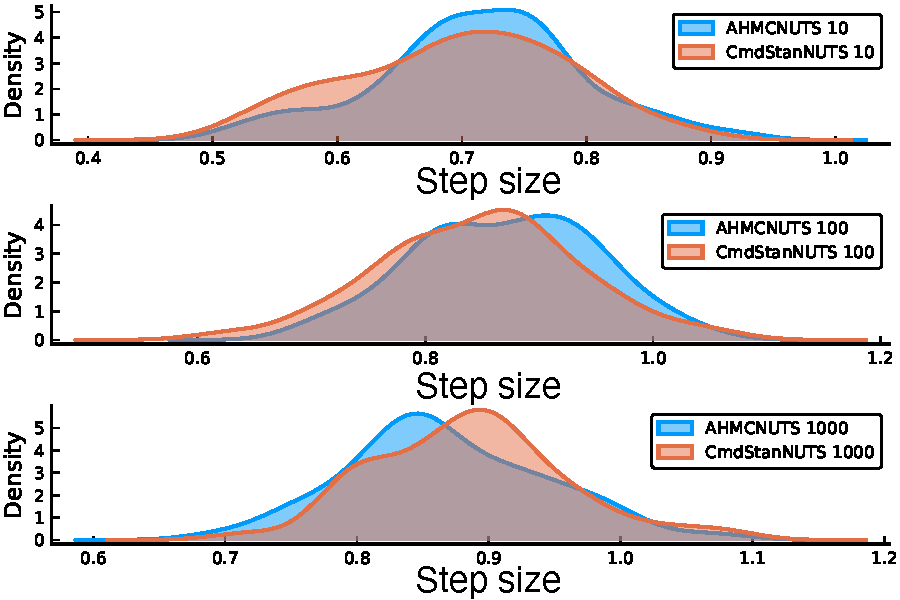
\includegraphics[width=0.33\textwidth]{images/Gaussian/density_epsilon.pdf}
    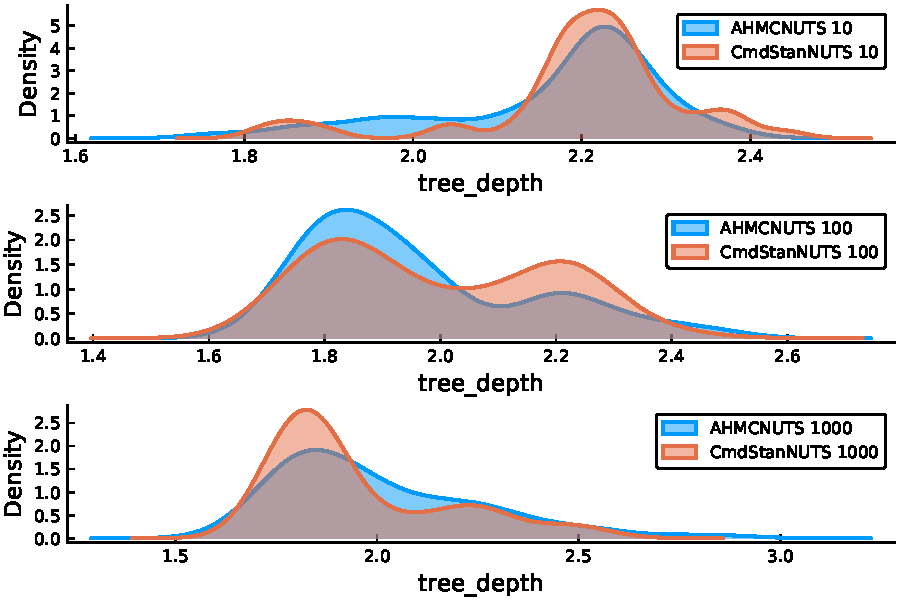
\includegraphics[width=0.33\textwidth]{images/Gaussian/density_tree_depth.pdf}
    \;\hfill
    \raisebox{\height}{\scalebox{0.73}{
        \begin{tabular}{lrrr}
            \toprule
            \multirow{2}{*}{} & \multirow{2}{*}{$N$} & \multicolumn{2}{c}{ESS} \\
            & & \multicolumn{1}{c}{$\mu$} & \multicolumn{1}{c}{$\sigma$} \\
            \midrule
            \texttt{Stan} & 10 & 513.163 & 466.577 \\
            \texttt{AHMC} & 10 & 503.535 & 447.722 \\
            \texttt{Stan} & 100 & 786.531 & 782.231 \\
            \texttt{AHMC} & 100 & 786.531 & 796.628 \\
            \texttt{Stan} & 1000 & 864.010 & 876.660 \\
            \texttt{AHMC} & 1000 & 832.255 & 844.452 \\
            \bottomrule
        \end{tabular}
    }}\hfill\;
    \caption{Gaussian (50 runs); left to right: step size, tree depth, ESS}
    \label{fig:gauss}
\end{figure}
\begin{figure}[h!]
    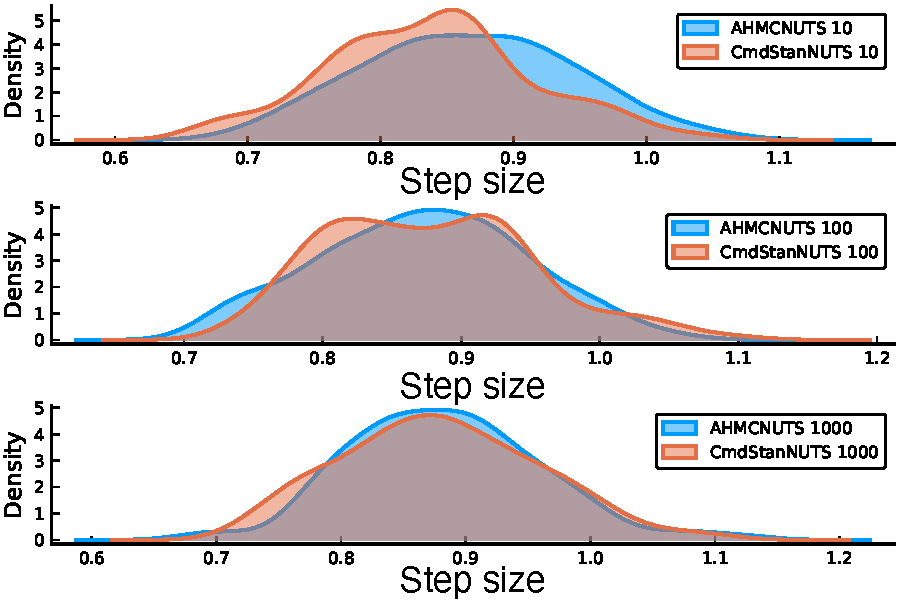
\includegraphics[width=0.33\textwidth]{images/SDT/density_epsilon.pdf}
    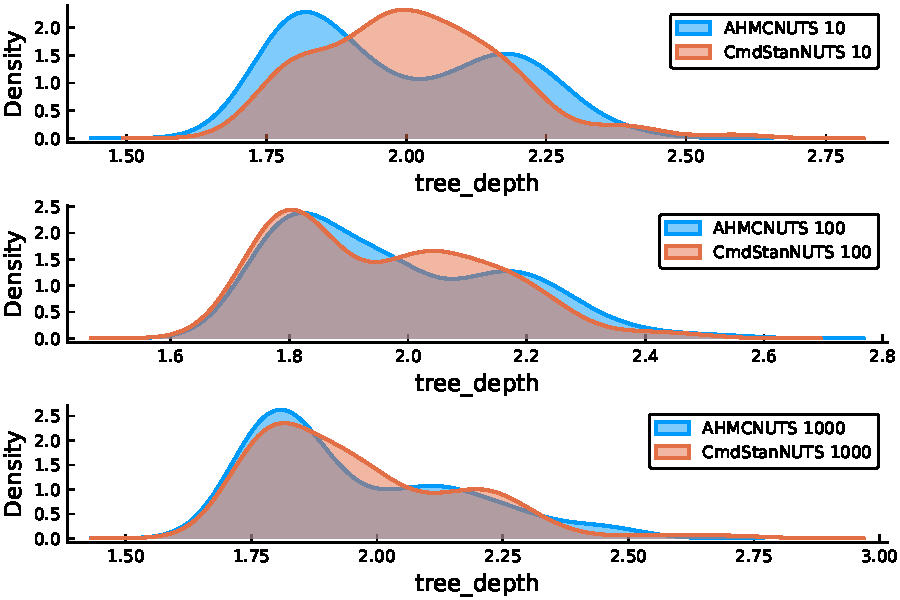
\includegraphics[width=0.33\textwidth]{images/SDT/density_tree_depth.pdf}
    \;\hfill
    \raisebox{\height}{\scalebox{0.73}{
        \begin{tabular}{lrrr}
            \toprule
            \multirow{2}{*}{} & \multirow{2}{*}{$N$} & \multicolumn{2}{c}{ESS} \\
            & & \multicolumn{1}{c}{$d$} & \multicolumn{1}{c}{$c$} \\
            \midrule
            \texttt{Stan} & 10 & 710.762  & 703.327 \\
            \texttt{AHMC} & 10 & 802.236 & 815.929 \\
            \texttt{Stan} & 100 & 820.741 & 823.152 \\
            \texttt{AHMC} & 100 & 814.308 & 846.357 \\
            \texttt{Stan} & 1000 & 844.478 & 872.961 \\
            \texttt{AHMC} & 1000 & 829.792 & 859.018 \\
            \bottomrule
        \end{tabular}
    }}\hfill\;
    \caption{SDT (100 runs); left to right: step size, tree depth, ESS}
    \label{fig:sdt}
\end{figure}
\begin{figure}[h!]
    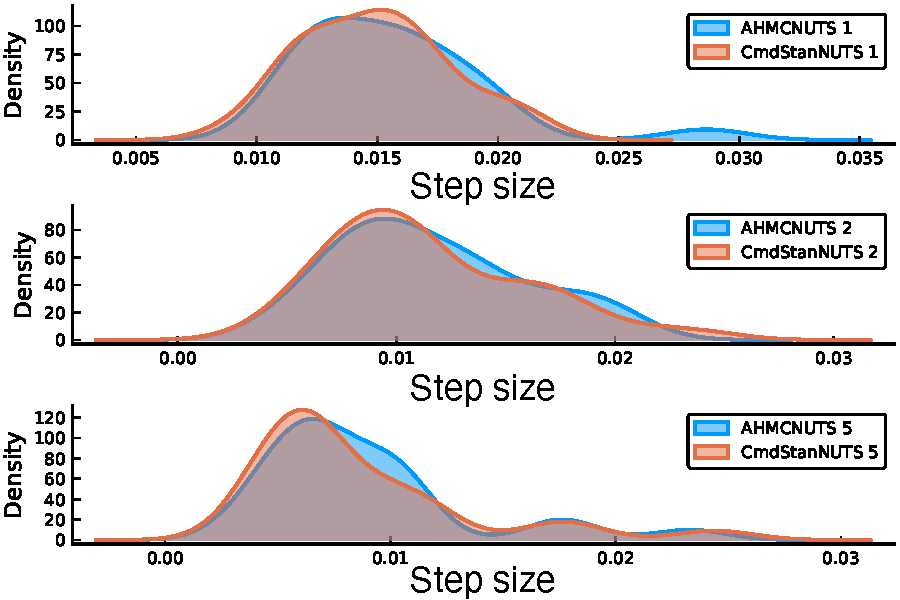
\includegraphics[width=0.3\textwidth]{images/Hierarchical_Poisson/density_epsilon.pdf}
    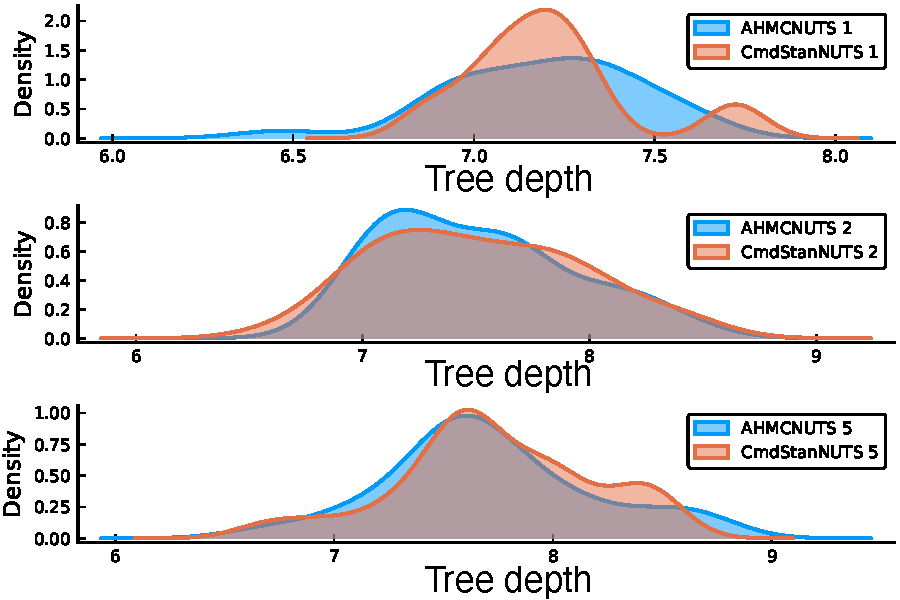
\includegraphics[width=0.3\textwidth]{images/Hierarchical_Poisson/density_tree_depth.pdf}
    \;\hfill
    \raisebox{\height}{\scalebox{0.69}{
        \begin{tabular}{lrrrr}
            \toprule
            \multirow{2}{*}{} & \multirow{2}{*}{$N$} & \multicolumn{3}{c}{ESS} \\
            & & \multicolumn{1}{c}{$a_0$} & \multicolumn{1}{c}{$a_1$} & \multicolumn{1}{c}{$b_\sigma$} \\
            \midrule
            \texttt{Stan} & 10 & 221.485 & 215.013 & 266.900 \\
            \texttt{AHMC} & 10 & 216.491 & 214.459 & 258.638 \\
            \texttt{Stan} & 20 & 208.286 & 207.041 & 241.080 \\
            \texttt{AHMC} & 20 & 206.458 & 200.469 & 236.546 \\
            \texttt{Stan} & 50 & 172.484 & 172.982 & 216.586 \\
            \texttt{AHMC} & 50 & 200.755 & 201.548 & 247.384 \\
            \bottomrule
        \end{tabular}
    }}\hfill\;
    \caption{HPR (25 runs); left to right: step size, tree depth, ESS (of some variables)}
\end{figure}
\begin{figure}[h!]
    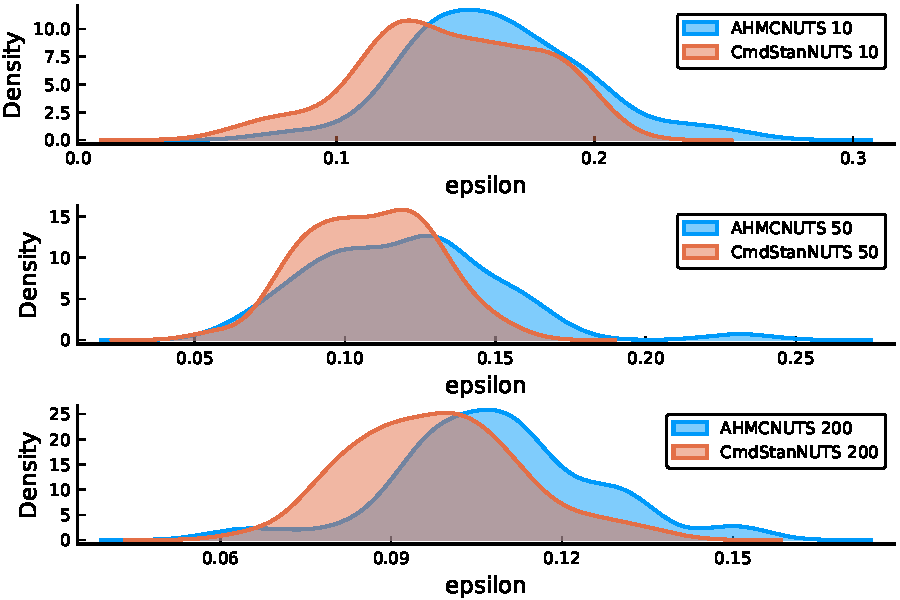
\includegraphics[width=0.3\textwidth]{images/LBA/density_epsilon.pdf}
    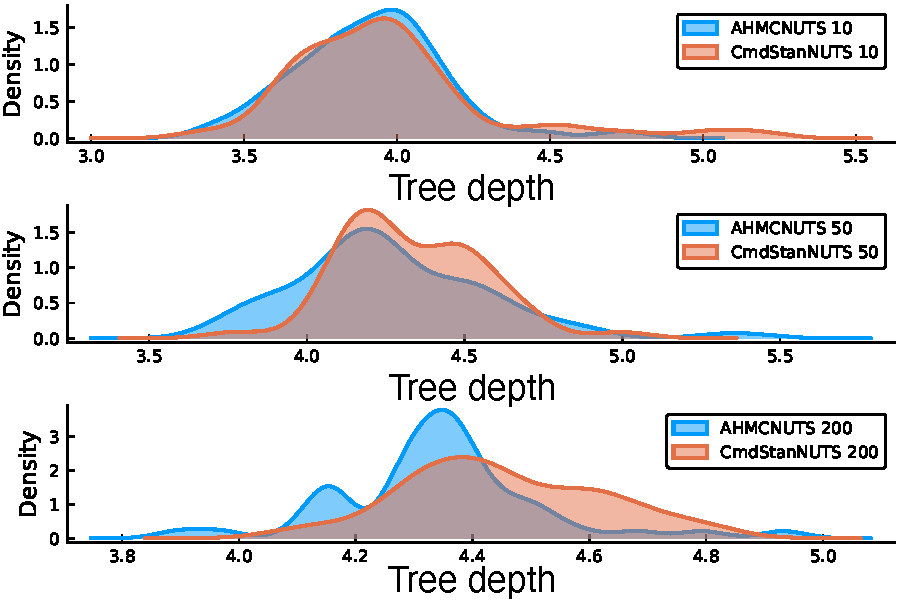
\includegraphics[width=0.3\textwidth]{images/LBA/density_tree_depth.pdf}
    \;\hfill
    \raisebox{\height}{\scalebox{0.69}{
        \begin{tabular}{lrrrrr}
            \toprule
            \multirow{2}{*}{} & \multirow{2}{*}{$N$} & \multicolumn{4}{c}{ESS} \\
            & & \multicolumn{1}{c}{$\tau$} & \multicolumn{1}{c}{$A$} & \multicolumn{1}{c}{$\nu_1$} & \multicolumn{1}{c}{$\nu_2$} \\
            \midrule
            \texttt{Stan} & 10 & 226.463 & 282.656 & 305.614 & 276.557 \\
            \texttt{AHMC} & 10 & 340.722 & 304.523 & 337.610 & 336.357 \\
            \texttt{Stan} & 50 & 212.838 & 238.003 & 24.009 & 232.667 \\
            \texttt{AHMC} & 50 & 248.249 & 238.979 & 248.331 & 255.421 \\
            \texttt{Stan} & 200 & 244.926 & 264.967 & 268.793 & 270.36 \\
            \texttt{AHMC} & 200 & 256.638 & 263.098 & 270.978 & 266.769 \\
            \bottomrule
        \end{tabular}
    }}\hfill\;
    \caption{LBA (50 runs); left to right: step size, tree depth, ESS (of some variables)}
    \label{fig:lba}
\end{figure}

\section{\turing~code for the linear regression model}
\label{app:turing-lr}
Below is the code snippet of running NUTS using \turing~for the LR model.
\lstinputlisting{lr.jl}

\end{document}
